% ब
\section{Insert} \label{s:results-insert}
% \newcommand{\Width}{0. 5\textwidth} \newcommand{\TB}[1]{\textbf{#1}} An
% \texttt{insert} operation triggers a referential integrity validation whenever
% a child entity containing foreign keys is inserted where the
% \texttt{ValidationHandler} validates that the foreign keys exist as primary
% keys in the parent entities.
Across all the solutions in the experiments,   \texttt{insert}  triggers a
validation when \texttt{Enrolment} entities are inserted as it is a child entity
containing foreign keys referencing to \texttt{Student} and \texttt{Course}.
On the other hand,  \texttt{Student} and \texttt{Course} entities have no
referential integrity constraints to be checked as these do not contain any
references to other column families.

The average response time and throughput for completing an \texttt{insert} on a
single entity for all the solutions is presented in Figure~\ref{fres:Insert}.
Specifically, Figure~\ref{fres:Insert-responsetime} shows the average time
consumed by the baseline and each solution to complete an \texttt{insert}
operation,  and Figure~\ref{fres:Insert-throughput} shows the  the number of
\texttt{insert} operations that can be completed in one second.

	\begin{figure}[H]
		\subfigure[Response time for Insert operation]
		{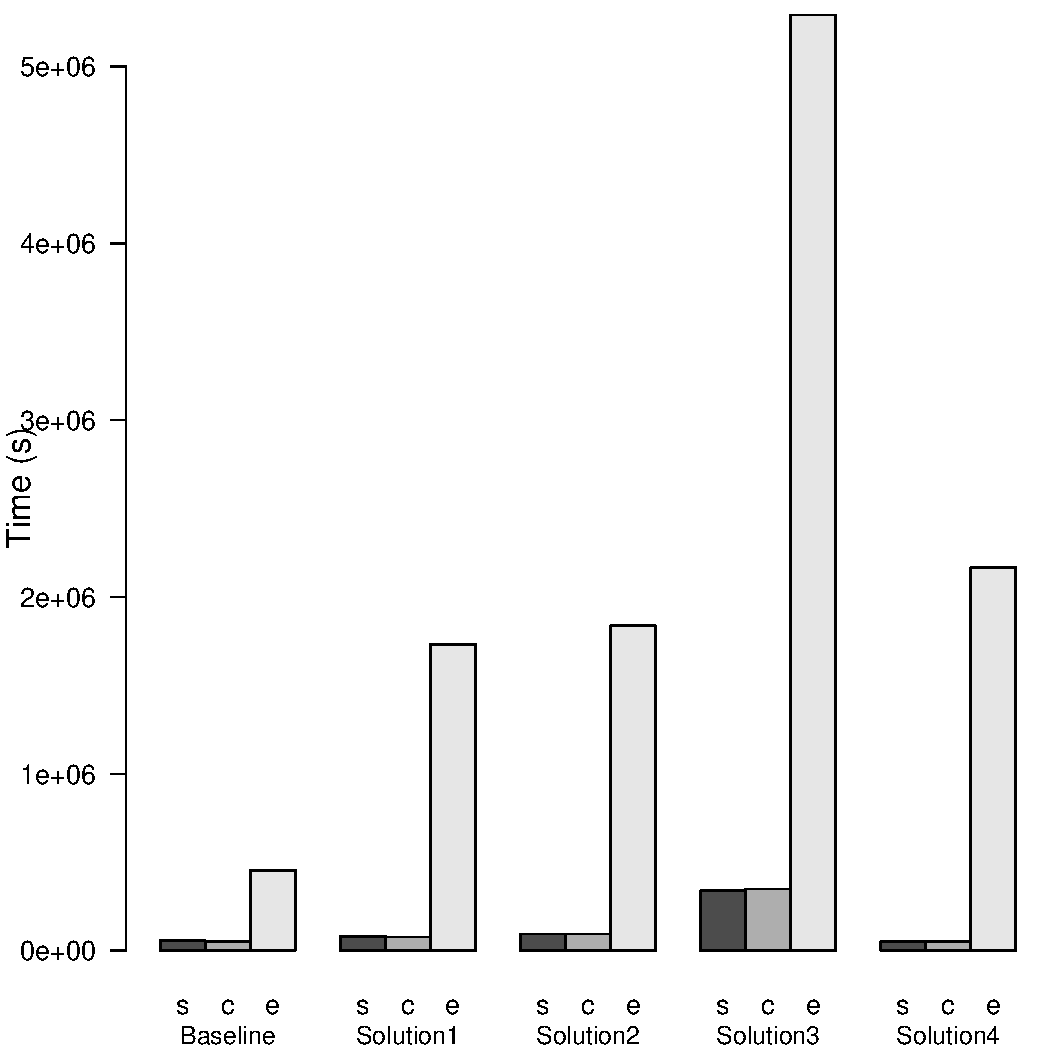
\includegraphics[width=\Width]{figure/result/barplot-insert-rt.pdf}\label{fres:Insert-responsetime}}
		\subfigure[Throughput for Insert operation]
		{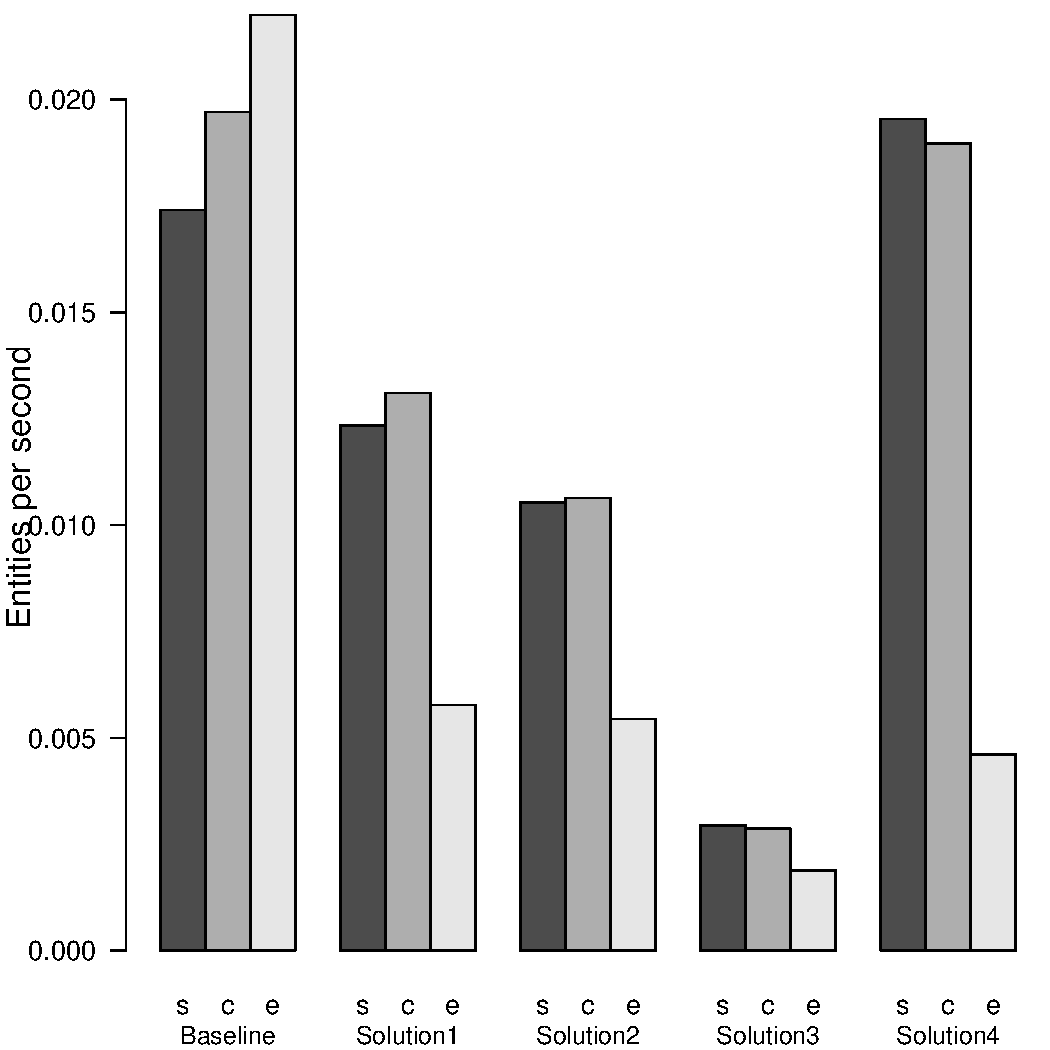
\includegraphics[width=\Width]{figure/result/barplot-insert-tp.pdf}\label{fres:Insert-throughput}}
		\caption{Performance of Solutions in Insert}\label{fres:Insert}
	\end{figure}
	
These results show that \texttt{insert} on a single entity of \texttt{Student}
and \texttt{Course} take approximately the same time to complete, and this is
consistent across solutions.  Inserting \texttt{Student} and \texttt{Course}
entities into their respective column families is faster than \texttt{insert} in
\texttt{Enrolment} because these are parent column families that have no
referencing constraints. Thus, the \texttt{insert} operation on these entities
involves only accessing the relevant \ac{FK} constraints from the metadata in
order to determine whether it is a parent or child entity.
% If the entity is a parent,  the validations are not triggered which is the
% case for \texttt{Student} and \texttt{Course} entities.
On the other hand,  \texttt{insert} on  \texttt{Enrolment}  takes the most time
in all the solutions as these entities have existing \ac{FK} constraints
indicating that they reference a parent entity which requires to retrieve
additional constraints. Moreover, its validation involves not only identifying
its relevant constraints but also accessing its parent column families
(\texttt{Student} and \texttt{Course}) to ensure that foreign keys match primary
keys. The results highlight the difference in response time when
foreign key validations are required in the case of \texttt{Enrolment}.
% the validation of one \texttt{Enrolment} entity and for other entities that do
% not have validations.
Note that these observations stand true across all the solutions.

More detailed information about the performance of each solution when
\texttt{insert} operations are performed is presented in
Figures~\ref{fres:insert-response-time} and~\ref{fres:insert-throughput}.
These figures show the average response time and throughput for the
\texttt{insert} operation on  each entity individually.
% Figure~\ref{fres:insert-user} presents the results for \texttt{insert} on a
% single \texttt{Student} entity in all the solutions.  Similarly
% Figures~\ref{fres:insert-course} and~\ref{fres:insert-enrolment} show the
% performance of \texttt{insert} on a \texttt{Course} and \texttt{Enrolment}
% entity in the solutions.
It can be seen that Solution~4 takes the least time to complete an 
\texttt{insert} on all the entities while Solution~3 takes the most time. 
Solution~4 takes the least time since it caches all the metadata thus avoiding 
multiple accesses to the \texttt{Metadata} column family, whereas Solution~3 
requires accessing \texttt{Metadata} each time a constraint is required. 
Regarding Solutions~1 and 2,  both perform similarly although Solution~2 takes 
slightly  more time than Solution~1 due to its additional search operation to 
locate the top row. Both the solutions are slightly slower than Solution~4 as 
constraints from these solutions are retrieved from the column family and  not 
from a cache. However, both solutions are faster than Solution~3 since 
retrieving constraints require no additional connections to access the metadata.




When compared to the baseline,  it is clear that the referential integrity
validations as well as metadata access caused the increased response time for
\texttt{insert} in all the solutions.  Since the validations are the same for
all solutions,  the performance differences in the solutions are due to the
different ways of accessing and processing the metadata.  From
Table~\ref{tres:ResponsetimeRatio}, Solutions~1 and 2  are almost 4 times slower
than the baseline, while Solution~3 is more than 11 times slower, and 
Solution~4 is almost 3 times slower than the baseline.
% Solution~3 takes the most time to perform one \texttt{insert} on all the
% entities.

Notice that when no referential integrity constraints need to be satisfied (e.g.
\texttt{Student} and \texttt{Course}), Solutions~1 and 2 are nearly 2 times
slower than the baseline,  Solution~3   more than 5 times slower, and  
Solution~4  almost similar to the baseline. Such differences are due to the
computational cost incurred while retrieving the metadata. 
% Note that the differences in the performance of the solutions is due to the
% distinctive way in which these store and acess metadata, as explained previously.
% A possible reason for this is that baseline operations are affected by the
% initialization as its \texttt{insert} operations are the very first operations
% to be executed.

\begin{landscape}
		\begin{figure}
		\centering
		\newcommand{\W}{.4\textwidth}
			\subfigure[Insert on Student]
			{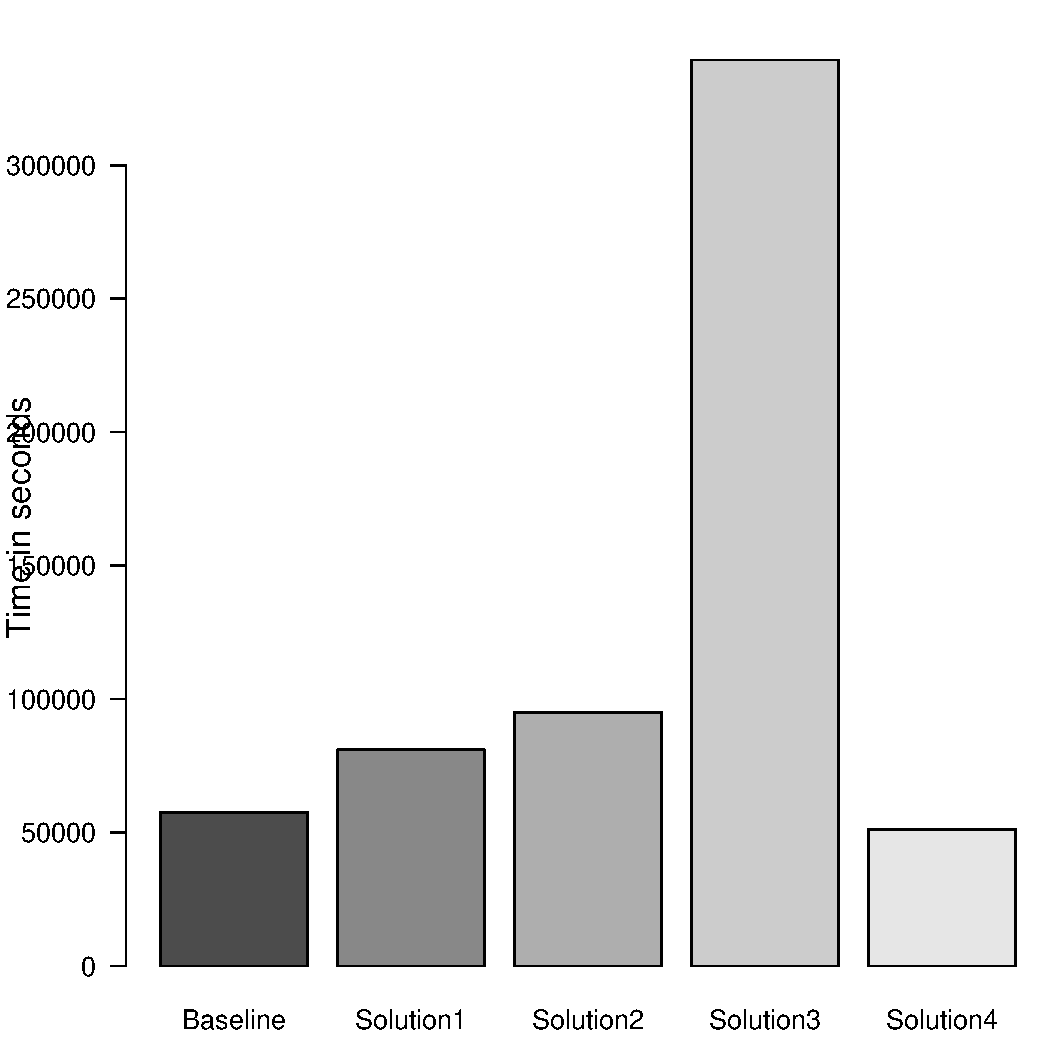
\includegraphics[width=\W]{figure/result/barplot-insert_student-rt.pdf}
			\label{fres:insert-user}}
			\subfigure[Insert on Course]
			{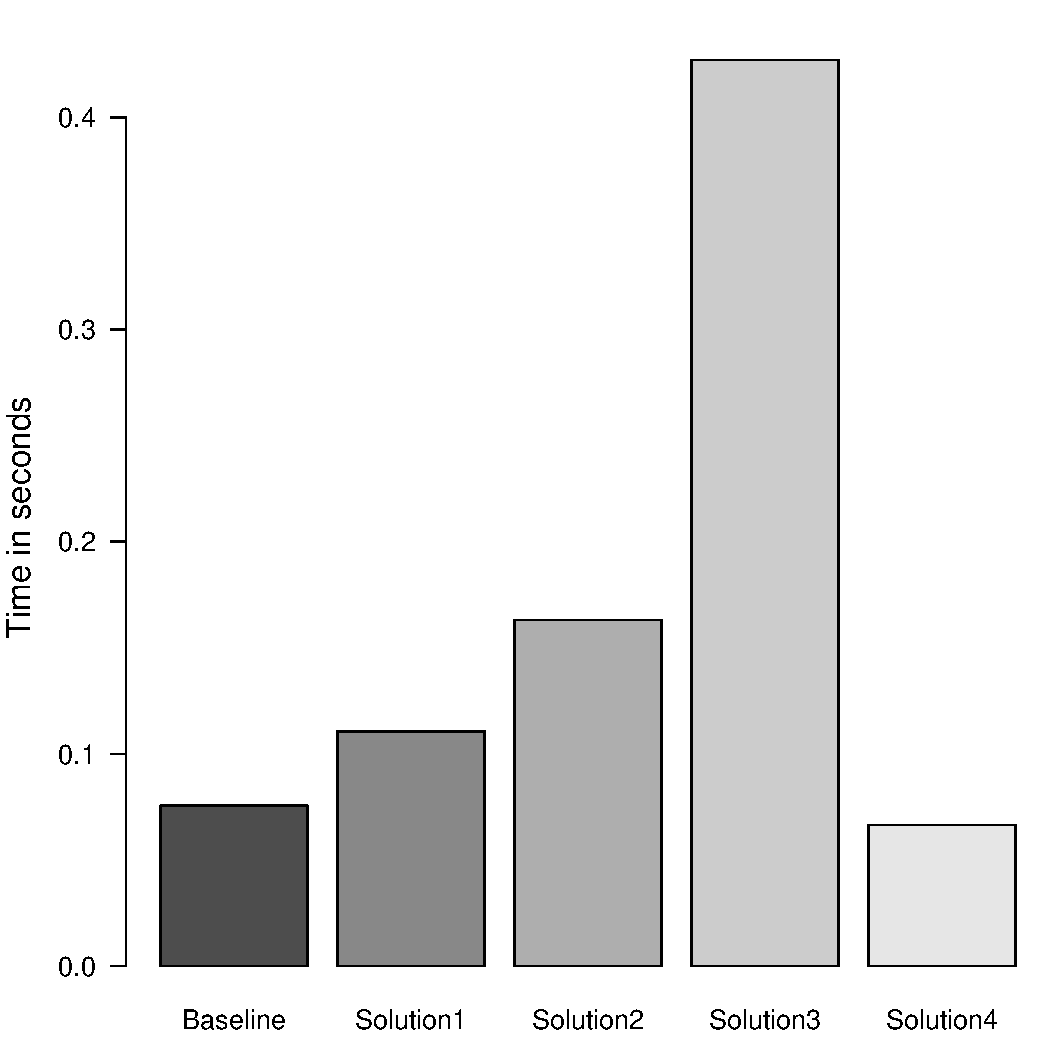
\includegraphics[width=\W]{figure/result/barplot-insert_course-rt.pdf}
			\label{fres:insert-course}}
			\subfigure[Insert on Enrolment]
			{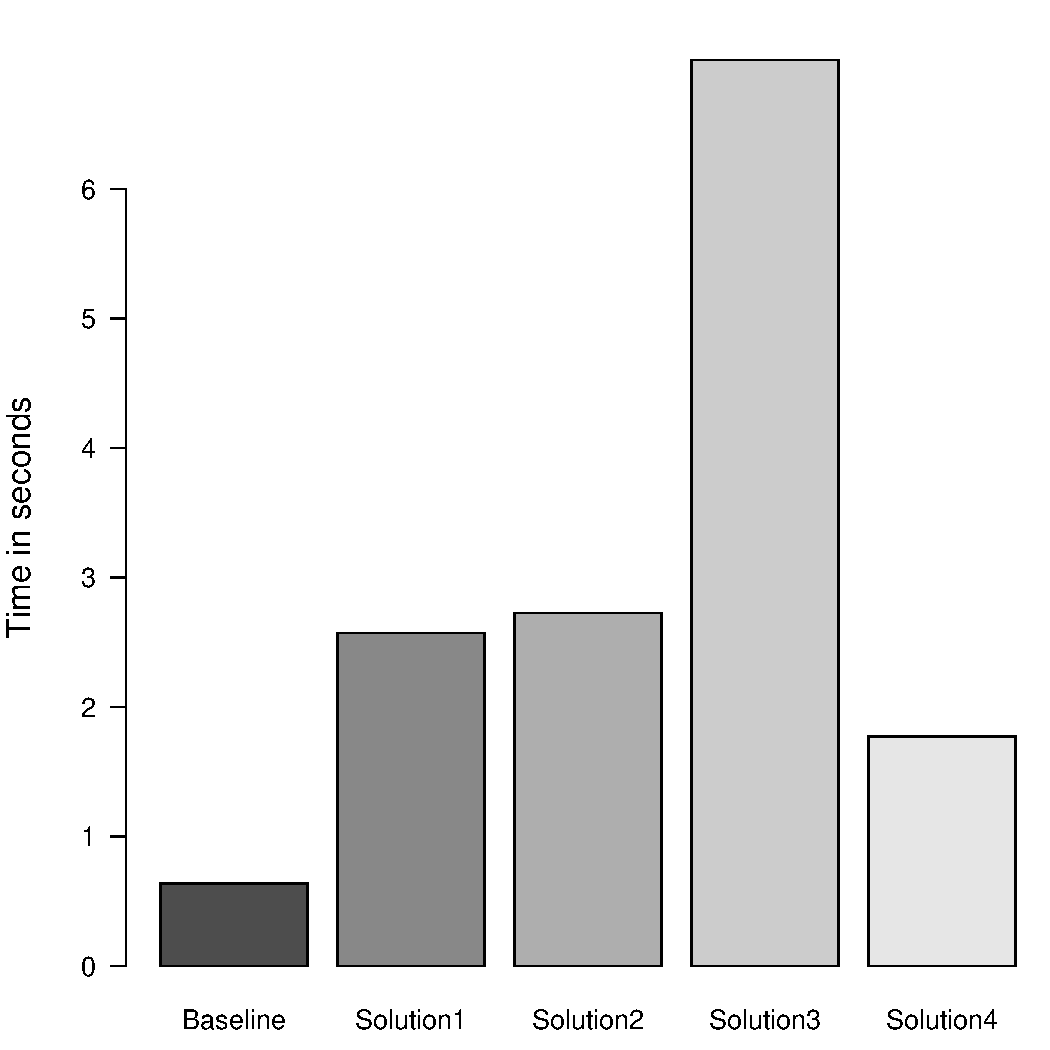
\includegraphics[width=\W]{figure/result/barplot-insert_enrolment-rt.pdf}}
			\caption{Response time inserting entities}\label{fres:insert-response-time}
			
			\subfigure[Insert on Student]
			{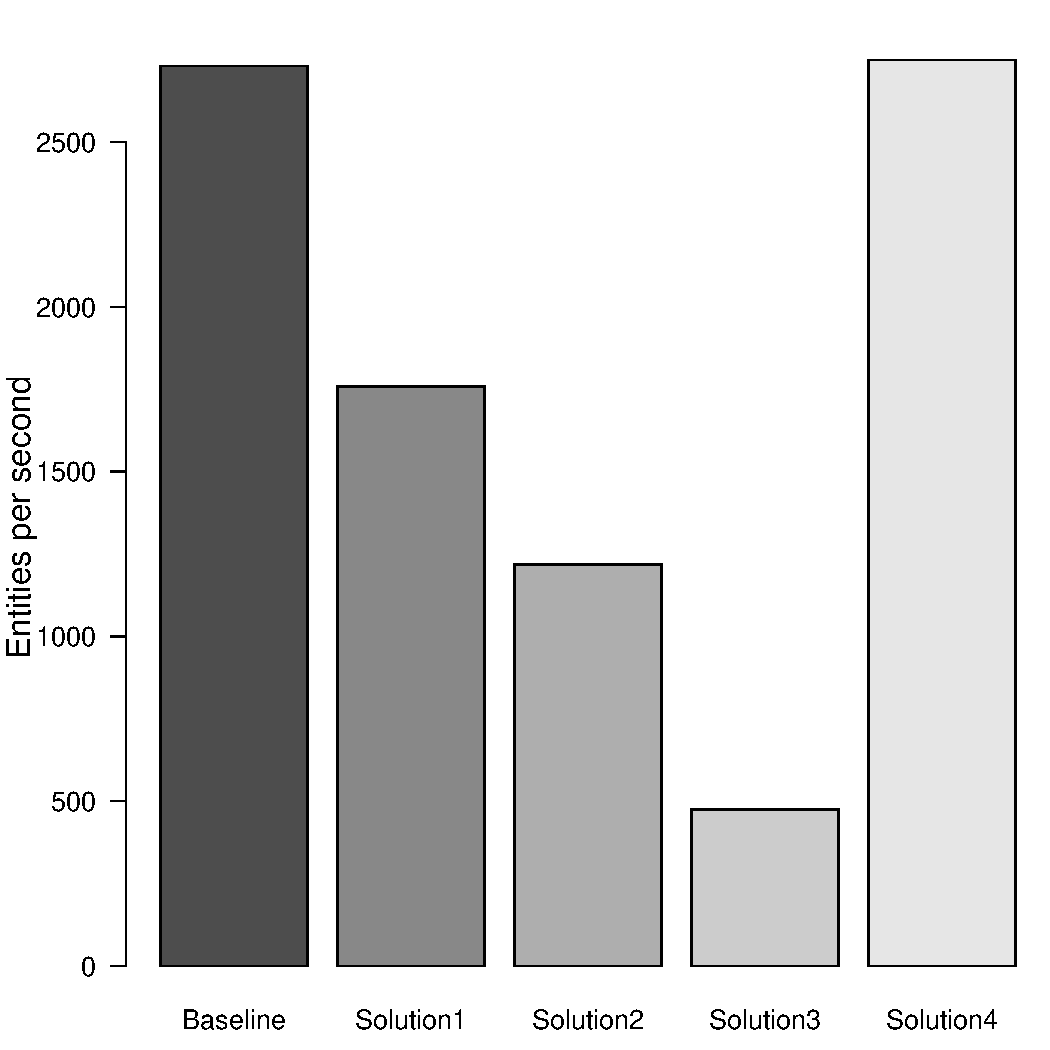
\includegraphics[width=\W]{figure/result/barplot-insert_student-tp.pdf}}
			\subfigure[Insert on Course]
			{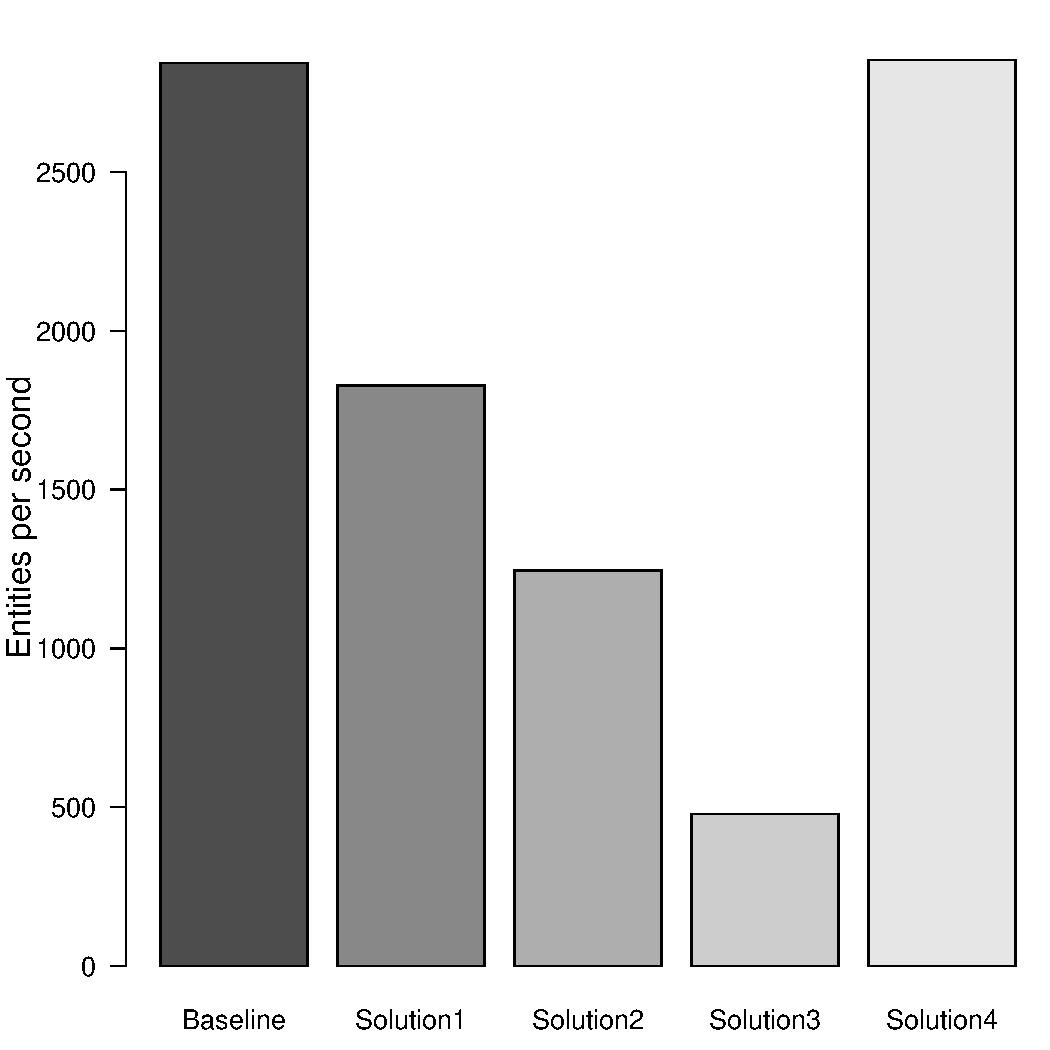
\includegraphics[width=\W]{figure/result/barplot-insert_course-tp.pdf}}			
			\subfigure[Insert on Enrolment]
			{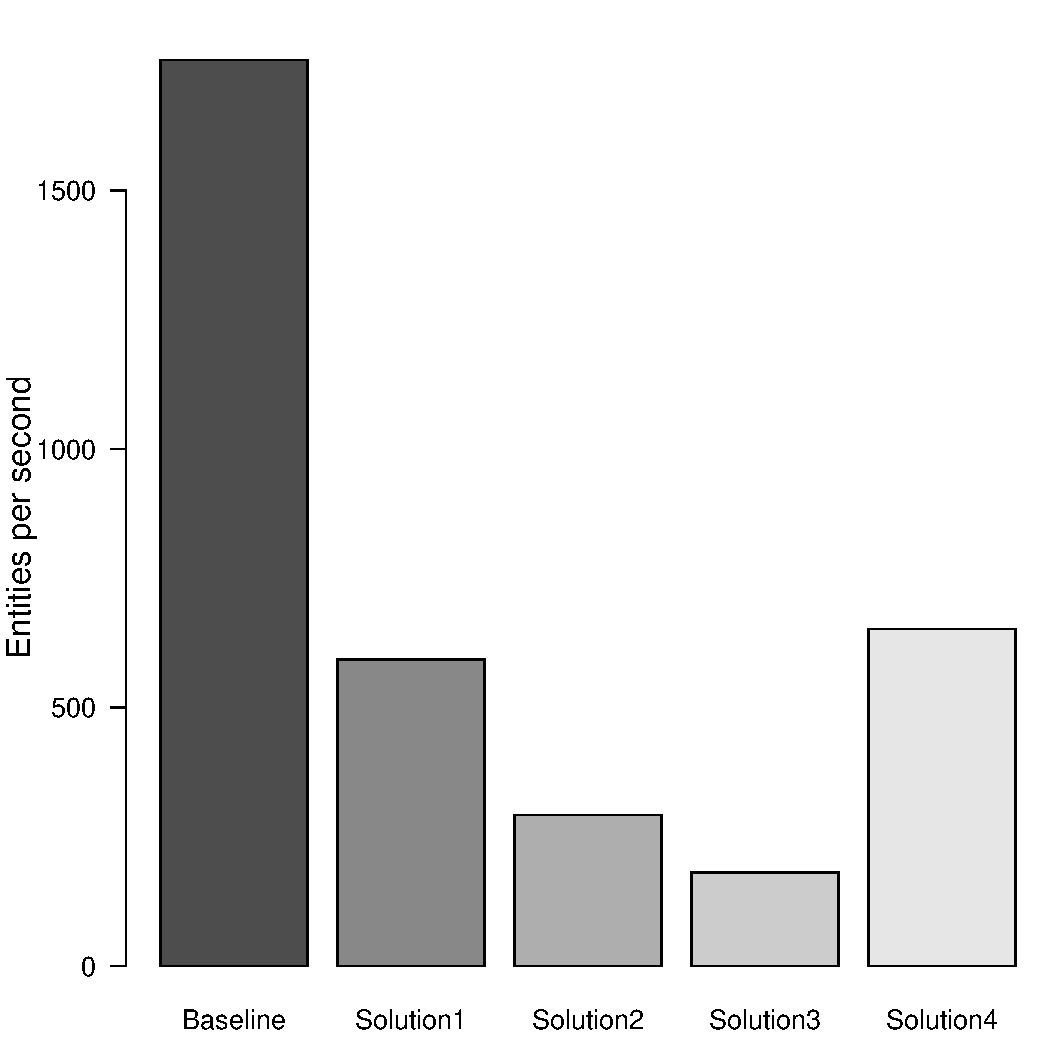
\includegraphics[width=\W]{figure/result/barplot-insert_enrolment-tp.pdf}}
			\caption{Throughput inserting entities}\label{fres:insert-throughput}
		\end{figure}
		
\end{landscape}
